\section{Interrupt}
E' un meccanismo genericamente implementato per gestire le periferiche, i dati arrivano in maniera aleatoria quindi stando a quanto conosciamo adesso dovremmo controllare periodicamente lo stato delle periferiche alla ricerca di un nuovo valore, questo è detto \emph{polling}.
Tuttavia è poco efficiente in quanto il tempo impiegato a controllare è tempo sprecato che potrei passare a fare altro quindi conviene solo su flussi di dati abbondanti in cui il \emph{success rate} delle interrogazioni è alto.
Inoltre se passa troppo tempo tra un controllo e l' altro i dati potrebbero essere troppo vecchi da utilizzare. 
Sarebbe bello essere notificati dalla periferica qualora avesse un nuovo valore per noi.

Per fare ciò ci vengono in aiuto le interruzioni (\emph{interrupts}), il nostro ATMega32 ha 3 sorgenti di interruzioni esterne: quando una periferica ha un valore lo segnala tramite un trigger specifico, al trigger il uC salta direttamente ad una parte del codice predisposta alla gestione di quel trigger.
Alla fine di questo codice, detto \emph{handler}, vi è una ret che permette di tornare al codice interrotto e riprendere l'esecuzione.

\begin{figure}[H]
    \centering
    
\includegraphics[width=150px]{images/15_Interrupt/interrupt_example.png}
\end{figure}

\subsection{Funzionamento}
Ognuno degli interrupt ha:
\begin{itemize}
    \item un flag di abilitazione: ENABLE bit
    \item un flag che indica se c'è un interrupt \emph{pendente}: FLAG bit
\end{itemize}
Quando arriva un evento viene settato il bit FLAG e se anche il bit ENABLE è attivato alla fine della prossima fase di esecuzione verrà eseguito il salto all' handler.
Quando viene effettuato il salto all' handler si disabilita anche il FLAG bit in quanto non si deve risaltare nuovamente all' handler finché non arriva un altro evento.

In fine c'è anche un bit generico per disabilitare tutte le interruzioni assieme, questo è il bit I all' interno dello SREG, se è disabilitato qualsiasi interruzione è disabilitata.
Questo flag viene disabilitato di default all' ingresso in un handler.

Gli indirizzi ai quali saltare in base all' interruzione sono hard-coded nel uC e sono quindi fissi.
Questi indirizzi coincidono con gli indirizzi delle righe della \emph{interrupt vector table} una tabella che va dall' indirizzo 0x0000 all' indirizzo 0x002a della FLASH. Abbiamo quindi 20 interruzioni diverse.

\begin{figure}[H]
    \centering
    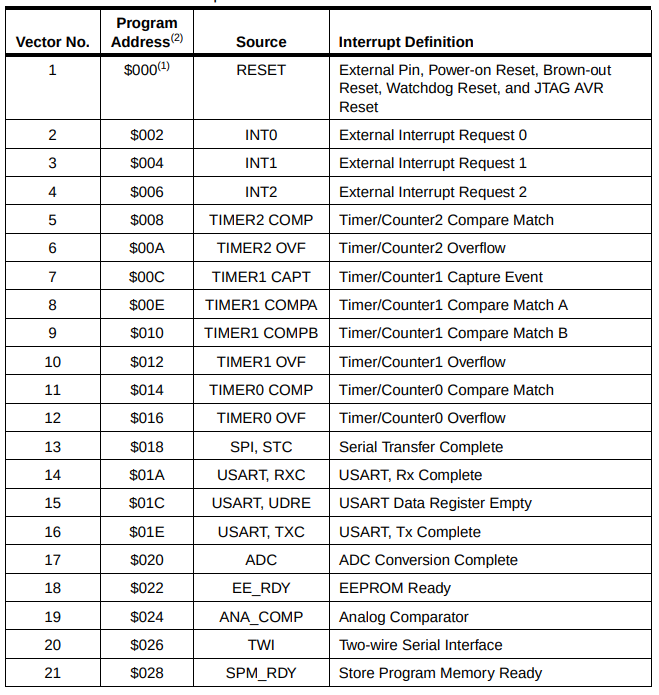
\includegraphics[width=300px]{images/15_Interrupt/interrupt_vector_table.png}
\end{figure}

Il codice delle interruzioni è direttamente in questa tabella, abbiamo quindi 32 bit di spazio per handler, abbastanza da poterci inserire una RJMP (1 riga) o una JMP (2 righe) ad una subroutine più grande.

\begin{figure}[H]
    \centering
    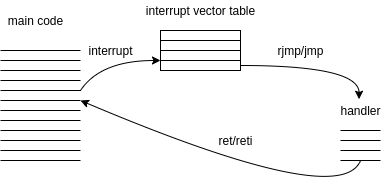
\includegraphics[width=250px]{images/15_Interrupt/interrupt_handler_with_table.png}
\end{figure}

NB: all' avvio le interruzioni sono tutte disabilitate, sia i singoli ENABLE bit che il flag I, questo perché bisogna prima di tutto abilitare lo stack altrimenti l' handler non potrà ritornare al codice.

NB: si noti che gli interrupt non salvano i registri ne i flag quando si entra, quindi bisogna creare procedure che non modifichino i registri ne i flag altrimenti il codice principale potrà fornire risultati sbagliati:
\begin{verbatim}
    push r0
    in r0, SREG
    push r0
        ; salva i flag sullo stack
    
    pop r0
    out SREG, r0
    pop r0
        ; ripristino i flag
\end{verbatim}

\subsubsection{Interrupt nidificati}
Abbiamo detto che all' entrata nell' handler il bit I viene disabilitato, questo fa si che tutte le interrzioni siano abilitate globalmente.
Se volessimo dare la possibilità di avere interrupt annidati dobbiamo abilitare il bit I a mano all' entrata dell' handler.

Bisogna fare molta attenzione a questi casi in quanto se gli interrupt avvengono troppo di frequente potrei non riuscire a finire quelli già iniziati e saturare lo stack di indirizzi di ritorno, inoltre il codice principale sarebbe eternamente bloccato!
\begin{verbatim}
    cli
        ; pone I a 0: disabilita le interruzioni
        
    sti
        ; pone I a 1: abilita le interruzioni
\end{verbatim}

Se invece all' interno di un handler ho le interruzioni disabilitate ma arriva un altro trigger da qualche perifericha il bit FLAG viene abilitato e vi rimane finché non decido di riabilitare le interruzioni e quindi servirlo.
In questo caso si parla di interrupt pendente.
Si noti che se ci sono più interrupt pendenti dello stesso tipo ne verrà gestito solo uno in quanto il flag non permette di contare quante volte è avvenuto l' evento.

Se invece ci sono più interrupt pendenti di tipo diverso quello che viene gestito prima è quello con indirizzo nella interrupt vector table minore.

\subsubsection{Ritorno dall' handler}
Per ritornare da un handler possiamo usare:
\begin{itemize}
    \item RET: semplicemente torna al chiamante prendendo l' indirizzo dallo stack
    \item RETI: oltre a tornare al chiamante abilita anche il flag I
\end{itemize}

\subsection{Interruzioni esterne}
Il package del uC ha 3 pin nominati INT0, INT1, INT2 che sono programmabili per recepire variazioni del segnale e lanciare interruzioni.
INT0 e INT1 sono praticamente identici mentre INT2 è più limitato nelle funzionalità in quanto introdotto successivamente.

\subsubsection{INT0 e INT1}
Possono essere programmati per lanciare un handler:
\begin{itemize}
    \item sul fronte di salita - \emph{rising edge}:
        \begin{figure}[H]
            \centering
            
\includegraphics[width=150px]{images/15_Interrupt/rising_edge.png}
        \end{figure}
        
    \item sul fronte di discesa - \emph{fallnig edge}:
        \begin{figure}[H]
            \centering
            
\includegraphics[width=150px]{images/15_Interrupt/falling_edge.png}
        \end{figure}

    \item su qualsiasi fronte:
        \begin{figure}[H]
            \centering
            
\includegraphics[width=150px]{images/15_Interrupt/each_edge.png}
        \end{figure}

    \item sul livello basso:
        \begin{figure}[H]
            \centering
            
\includegraphics[width=150px]{images/15_Interrupt/low_level.png}
        \end{figure}
        Questa modalità è particolarmente utile per eseguire un multiplexing degli interrupt esterni: supponiamo che 3 interrupt non ci bastino, posso configurare la detection sul livello basso ed usare questo circuito:
        \begin{figure}[H]
            \centering
            
\includegraphics[width=150px]{images/15_Interrupt/interrupt_multiplexing.png}
        \end{figure}
        Ho quindi due sorgenti di interruzioni A e B che vanno in una porta NOR e finché almeno uno dei 2 è alto l' uscita  della porta sarà bassa.
        Avendo la rilevazione sul livello logico 0 detecto questa condizione, salto all' handler disabilitando le interruzioni, interrogo le periferiche per vedere quella che mi ha chiesto di essere gestita, la gestisco e porrà a 0 la sua richiesta. Pulisco infine il FLAG bit a mano e ritorno dall' handler.
        Se anche l' altra periferica vuole essere gestita allora subito dopo aver pulito il FLAG bit esso verrà nuovamente riattivato e quindi partirò gestendo la seconda interruzione.
\end{itemize}

Per abilitare uno dei due interrupt si deve prima configurare la modalità di utilizzo all' interno del registro MCUCR:
\begin{figure}[H]
    \centering
    
\includegraphics[width=320px]{images/15_Interrupt/MCUCR.png}
\end{figure}
\begin{itemize}
    \item ISC01:ISC00: indicano la modalità di funzionamento dell' interrupt 0
    \item ISC11:ISC10: indicano la modalità di funzionamento dell' interrupt 1
\end{itemize}
le modalità sono codificate:
\begin{table}[ht!]
    \centering
    \begin{tabular}{c|c|l}
        ISCX1 & ISCX0 & modalità \\
        \hline
        0 & 0 & livello basso \\
        0 & 1 & qualsiasi variazione \\
        1 & 0 & falling edge \\
        1 & 1 & rising edge \\
    \end{tabular}
\end{table}

Es: INT1 sul falling edge e INT0 su qualsiasi variazione:
\begin{verbatim}
    ldi r16, (1 << ISC11)|(1 << ISC00)
    out MCUCR, r16
        ; NO! sovrascrivo anche i bit che
        ; magari non voglio toccare
    
    in r16, MCUCR
    ori r16, (1 << ISC11)|(1 << ISC00)
    out MCUCR, r16
        ; cambio solo i bit necessari
\end{verbatim}

\subsubsection{INT2}
Ha solo un bit di controllo localizzato in MCUCSR:
\begin{figure}[H]
    \centering
    
\includegraphics[width=320px]{images/15_Interrupt/MCUCSR.png}
\end{figure}
le modalità sono codificate:
\begin{table}[ht!]
    \centering
    \begin{tabular}{c|l}
        ISC2 & modalità \\
        \hline
        0 & falling edge \\
        1 & rising edge \\
    \end{tabular}
\end{table}

\subsubsection{Abilitazione interrupt}
Una volta configurata la modalità di funzionamento si devono abilitare i singoli interrupt, per fare ciò abbiamo 3 flag nel registro GICR:
\begin{figure}[H]
    \centering
    
\includegraphics[width=320px]{images/15_Interrupt/GICR.png}
\end{figure}
posto 1 in uno degli slot abilita l'interrupt corrispondente.

\subsubsection{Bit di interrupt pendente}
I bit di interrupt pendente sono nel registro GIFR:
\begin{figure}[H]
    \centering
    
\includegraphics[width=320px]{images/15_Interrupt/GIFR.png}
\end{figure}
per pulirli bisogna scriverci 1 mentre può settarli solo l' hardware.

\subsection{Esempio di programma}
\begin{verbatim}
    .include "m32def.h"
    reset:
        rjmp start
    
    .org 0x0001
    int0_vect:
        rjmp int0_handler
    
    .org 0x002a
    start:
            ; abilitiamo lo stack che ci 
            ; serve per le interruzioni
        ldi r16, low(RAMEND)
        ldi r17, high(RAMEND)
        out spl, r16
        out sph, r17
        
            ; impostiamo interrupt INT0
            ; su fronte di salita
        in r16, MCUCR
        ori r16, (1 << ISC01)|(1 << ISC00)
        out MCUCR, r16
            ; abilitiamo INT0
        in r16, GICR
        ori r16, (1 << INT0)
        out GICR, r16
            ; abilito le interruzioni
            sei
        
        ; yadda-yadda
        
    end:
        rjmp end
    
    
    int0_handler:
        ; codice dell' interrupt
        reti
\end{verbatim}

\subsection{Sezione critica}
Supponiamo di avere il segunte codice:
\begin{verbatim}
    add yl, xl
    adc yh, xh
\end{verbatim}
se una interruzione avviene tra la prima e la seconda potrei perdere il carry bit.
Questa è una sezione critica che quindi va eseguita in maniera \emph{atomica}.
Un codice più sicuro sarebbe ad esempio:
\begin{verbatim}
    cli         ; disabilito le interruzioni
    add yl, xl
    adc yh, xh
    sei         ; abilito le interruzioni
\end{verbatim}
l' interrupt è ritardato di qualche ciclo di clock, se la sezione critica è molto piccola va bene usare questo approccio.

Tuttavia c' è un problema:
\begin{itemize}
    \item se all' inizio della sezione critica $I=1$ allora l' uscita è coerente
    \item se all' inizio della sezione critica $I=0$ allora alla fine abbiamo attivato le interruzioni, probabilmente senza volerlo
\end{itemize}
una soluzione più generica è pertanto:
\begin{verbatim}
    in r0, SREG
    cli
        ; salvo i flag e disabilito le interruzioni
    add yl, xl
    adc yh, xh
    out SREG, r0
        ; rimetto i flag al loro posto
\end{verbatim}

Se si vuole essere ancora più raffinati possiamo usare delle macro:
\begin{verbatim}
    .macro save_irq
        in r0, SREG
        cli
    .endmacro
    
    .macro restore_irq
        out SREG, r0
    .endmacro
    
    save_irq
    add yl, xl
    adc yh, xh
    restore_irq
\end{verbatim}

Un' altra opzione è quella di creare handler che non modifichino flag e registri, ma questa soluzione non è universale in quanto a volte bisogna eseguire operazioni con un timing particolare quindi oltre al contenuto dei flag e registri importa anche il numero di cicli di clock impiegati tra le istruzioni.